% !TEX root = ../my-thesis.tex
%
\chapter{Proton-proton collision phenomenology}
\label{sec:pp}

\section{Basic concepts}
\label{sec:pp:basics}
Collisions of protons at high energy scales can be described by perturbative quantum field theory. Matrix elements of strong interaction processes can be calculated systematically at fixed orders in the strong coupling constant \(\alpha_{s}\). However, the description of \HepProcess{\Pp\Pp} collision events involves additional complexity, as protons are strongly interacting and composite objects. In \HepProcess{\Pem\Pep} collisions, the participants in the scattering process are the same elementary particles which are accelerated. In contrast, in a typical \HepProcess{\Pp\Pp} collision, it is the proton beams which are accelerated but two partons which take part in the hard scattering process. The debris of the initial protons gives rise to additional activity in the event.
Furthermore, the interactions which convert the coloured parton states into hadrons occur at low momentum scale, where the strong coupling becomes large, and consequently, they cannot be described by perturbation theory.

The detailed description of a \HepProcess{\Pp\Pp} collision event can be decomposed into various processes. \Cref{fig:pp:collision} shows a proton-proton collision event with the production of a top quark pair and a Higgs boson in the hard scattering process. The various colours encode different processes, which are listed ordered by the respective momentum transfer \(Q^2\), starting with the hardest process.
\begin{figure}[htbp]
	\centering
	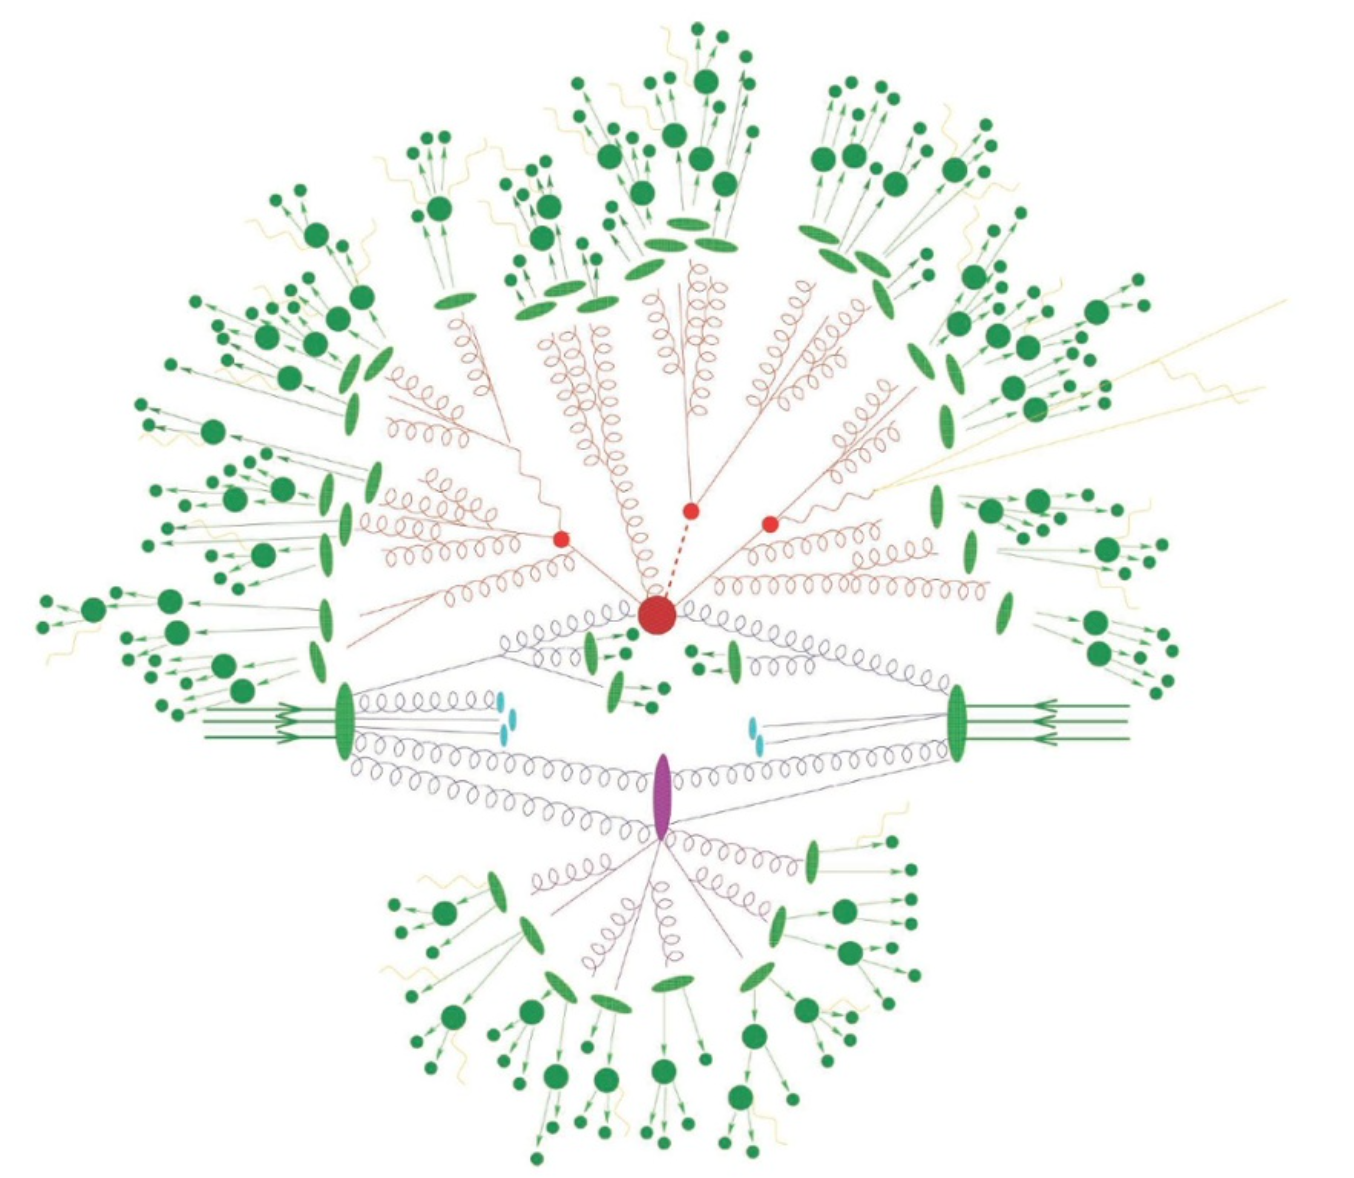
\includegraphics[width=0.95\textwidth]{figures/protoncollisions/pp-event.png}
	\caption{Sketch of a proton-proton collision event in which a top quark pair and a Higgs boson are produced in the hard scattering process. The incoming protons are shown as the central green ellipses with three incoming valence quark lines. The hard scattering process is depicted as the central red blob. The initial and final state radiation processes are shown in blue and red, respectively. The underlying event of other partons scattering and producing further activity is shown in purple. All emerging partons undergo hadronisation, resulting in cascading showers of hadrons, which are shown in green. Figure reproduced from Ref.~\cite{Campbell2018}.}
	\label{fig:pp:collision}
\end{figure}
\begin{enumerate}
	\item Hard interaction (red)
	\item Initial state radiation (ISR) (blue)
	\item Final state radiation (FSR) (red)
	\item Hadronisation and hadron decays (green)
	\item Underlying event (purple)
\end{enumerate}

The hard scattering process involves the largest momentum scales, allowing for a description at fixed-order perturbation theory in QCD. The description of the hard scattering process includes the relevant features of the event, such as the production of heavy states or hard QCD jets. Typically, the description of the hard scattering process is achieved by automated evaluation of the relevant Feynman diagrams and numerical integration over the phase-space of the final state particles.
Secondary emissions include ISR from the incident partons and FSR from the particles produced in the hard scattering process. The ISR originates from the breakdown of the coherent quantum states initiated by the parton taking part in the hard interaction. The FSR is due to Bremsstrahlung of particles produced in the hard scattering process, which results in the emission of particles at lower scales. The emitted QCD radiation initiates a parton shower via parton fragmentation, c.f. the splitting processes \HepProcess{\Pq \to \Pq \Pgluon}, \HepProcess{\Pgluon \to \Pgluon \Pgluon}, and \HepProcess{\Pgluon \to \Pq \Paq}. As the result of the parton shower, a set of coloured partons at the scale of a few \si{\giga\electronvolt} emerges. At this momentum scale, confinement becomes relevant, and the coloured parton states break up into a primary generation of colour-neutral hadrons. This process is called hadronisation. The description of this process involves simulation in non-perturbative models. The most prominent models are the Lund string model~\cite{Andersson1983} and the cluster model~\cite{Webber1984,Marchesini1988,Marchesini1992}. These initial hadrons decay further in cascades of hadrons, resulting in the formation of QCD jets.
The underlying event refers to multi-parton interactions in the event, which are difficult to model. Typically, the momentum transfer in these additional parton interactions is soft compared to the hard interaction. The description of the underlying event employs models with tunable parameters.

\section{Parton density functions}
\label{sec:pp:pdfs}
A key insight of the parton model is that the quarks and gluons inside a proton can be described in terms of parton density functions (PDFs) \(f_{a / \Pp}(x, Q^2)\) that parametrise the probability of finding a parton \(a\) with momentum fraction \(x\) at a scale of \(Q^2\) inside a proton.
PDFs can be measured in different processes and at different scales. These can be related to each other by the Dokshitser-Gribov-Lipatov-Altarelli-Parisi (DGLAP) equations~\cite{Dokshitzer1977,Gribov1972,Altarelli1977}
\begin{align}
    \frac{\partial}{\partial \log Q^2} \begin{pmatrix} f_{q/\Pp}(x, Q^2) \\ f_{g/\Pp}(x, Q^2) \end{pmatrix} = \frac{\alpha_{s}(Q^2)}{2\pi} \int_{x}^{1} \frac{\dd{z}}{z} \begin{pmatrix} \mathcal{P}_{qq}(\frac{x}{z}) \mathcal{P}_{qg}(\frac{x}{z}) \\ \mathcal{P}_{gq}(\frac{x}{z}) \mathcal{P}_{gg}(\frac{x}{z}) \end{pmatrix} \begin{pmatrix} f_{q / \Pp} (z, Q^2) \\ f_{g / \Pp} (z, Q^2) \end{pmatrix}.
\end{align}
The splitting functions \(\mathcal{P}_{gg}(\frac{x}{z})\) can be expanded in perturbation theory and are listed, for instance, in Ref.~\cite{Campbell2018}.

The PDFs can be determined from fits to a wide range of experimental data. In typical PDF fits, about \num{3000} data points are used ~\cite{Campbell2018}, including deep inelastic scattering data from fixed-target experiments and the HERA electron-proton collider, and data from Drell-Yan and jet production processes at the Tevatron and the Large Hadron Collider. The CT14~\cite{Dulat2016}, MMHT2014~\cite{HarlandLang2015}, and NNPDF3.0~\cite{Ball2015} PDF sets are the primary choices to describe proton-proton collisions at the Large Hadron Collider~\cite{Butterworth2016} and provide PDFs at leading order (\LO), next-to-leading order (\NLO) and next-to-next-to-leading order (\NNLO) precision in \(\alpha_{s}\).

\Cref{fig:pp:pdfs:ct14} shows the PDFs from the CT14 PDF set for the scales \(Q^2 = \SI{2}{\square\giga\electronvolt}\) and \(Q^2 = \SI{100}{\square\giga\electronvolt}\). The proton valence quark PDFs (\Pqu and \Pqd) are the largest for high \(x\)-values, while the sea-quark and gluon PDFs dominate at low \(x\)-values. For higher scale \(Q^2\), the gluon and sea-quark contributions are enhanced together with the valence quarks at low \(x\)-values, as more parton structure is resolved.
\Cref{fig:pp:pdfs:comparison} shows a comparison of the CT14 PDF set to the MMHT2014 and NNPDF3.0 PDF sets with their respective uncertainty bands. The discrepancies between different PDF sets originate from different input data, different choices for the parameters and PDF parametrisation.

\begin{figure}[htbp]
	\centering
    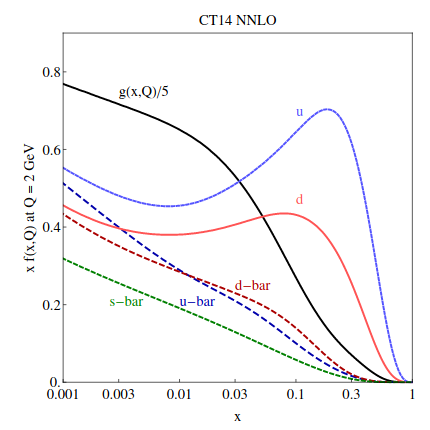
\includegraphics[width=.75\textwidth]{figures/protoncollisions/pdf_ct14_q2.png} \\
    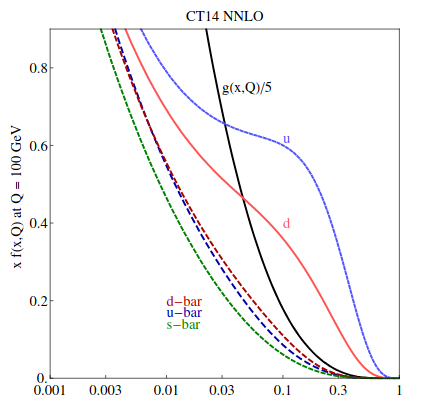
\includegraphics[width=.75\textwidth]{figures/protoncollisions/pdf_ct14_q100.png}
    \caption{The CT14 parton distribution functions at the scales of \SI{2}{\giga\electronvolt} (top) and \SI{100}{\giga\electronvolt} (bottom) for \Pqu \Paqu, \Pqd, \Paqd, \Paqs, and \Pgluon. Figure reproduced from Ref.~\cite{Dulat2016}.}
    \label{fig:pp:pdfs:ct14}
\end{figure}

\begin{figure}[htbp]
    \centering
    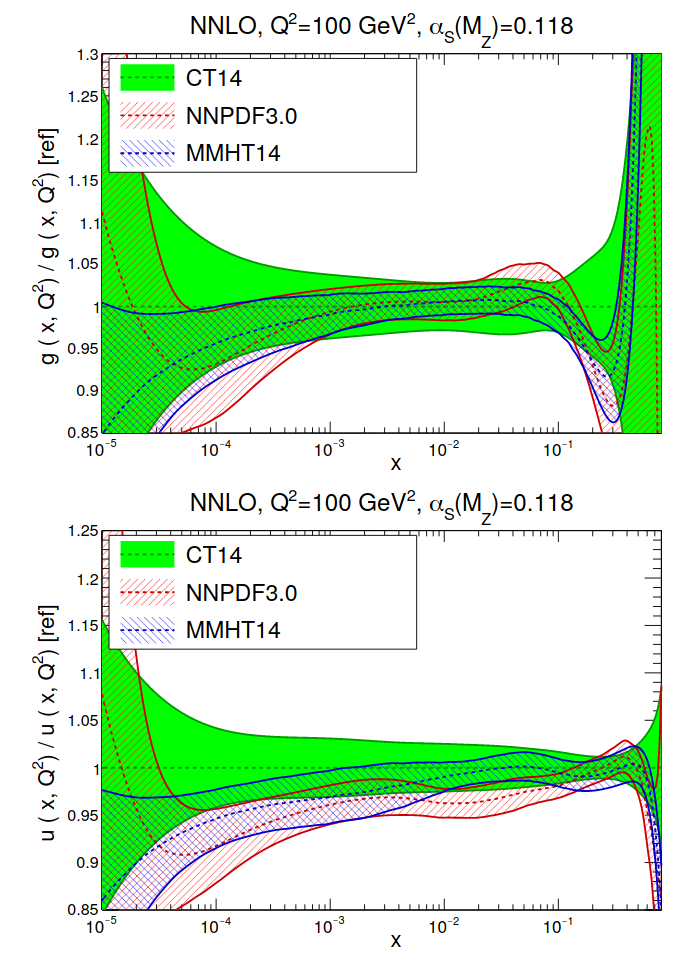
\includegraphics[width=.95\textwidth]{figures/protoncollisions/pdf_comparison.png}
    \caption{Comparison of the gluon (top) and up quark (bottom) PDFs from the CT14, MMHT14 and  NNNPDF3.0 sets at next-to-next-to-leading order (\NNLO) at a scale of \(Q^2= \SI{100}{\square\giga\electronvolt}\). The results are shown relative to the central value of CT14. Figure reproduced from Ref.~\cite{Butterworth2016}.}
    \label{fig:pp:pdfs:comparison}
\end{figure}


\section{Calculation of cross-sections}
\label{sec:pp:crosssections}
According to factorisation theorems~\cite{Collins1989}, the total cross-section for any process \HepProcess{\Pproton \Pproton \to X} can be written as a sum over the partonic cross-sections \(\hat{\sigma}_{\HepProcess{a b \to X}}\) for all parton types \(a\) and \(b\)
\begin{align}
    \sigma_{\HepProcess{\Pproton \Pproton \to X}} = \sum_{a} \sum_{b} \int_{0}^{1} \dd{x_{1}} \int_{0}^{1} \dd{x_{2}} f_{a}(x_1, \muF) f_{b}(x_2, \muF) \hat{\sigma}_{\HepProcess{a b \to X}}(x_{1} p_{1}, x_{2} p_{2}, \muF, \muR).
\end{align}

The PDFs in proton-proton collisions evolve with the factorisation scale \(\muF\) according to the same non-perturbative interactions that give rise to scaling violations in deep inelastic scattering. The renormalisation scale \(\muR\) is another process-dependent quantity, which indicates the scale at which the coupling constants are evaluated. Typical choices for \(\muF\) and \(\muR\) are dictated by one hard scale \(Q^2\) of the process like the mass of an \(s\)-channel resonance of mass \(M\), such that \(\muF = \muR = Q^2 = M^2\).

As the momentum of the partons is distributed according to the PDFs, the centre-of-mass frame of the process is unlikely to coincide with the laboratory frame of reference. In the parton model, one parton has momentum \(p_{z_{1}} = x_{1} \sqrt{s} / 2\) in the detector frame, while the other has the momentum \(p_{z_{2}} = - x_{2} \sqrt{s} / 2\), where \(\sqrt{s}\) is the centre-of-mass energy of the proton-proton-system. In the partonic centre-of-mass frame, the energy of the parton is \(\hat{s} = x_1 x_2 s\) and it has net momentum along the beam axis of \(\hat{p}_{z} = (x_1 - x_2)\).

The partonic cross-section in the limit of massless partons
\begin{align}
    \hat{\sigma}_{\HepProcess{a b \to X}}(x_{1} p_{1}, x_{2} p_{2}, \muF, \muR) = \frac{1}{2\hat{s}} \int \dd{\Phi_{n}} \abs{\mathcal{M}_{\HepProcess{a b \to X}}}^2 (\Phi_{n}, \muF, \muR)
\end{align}
can be evaluated in perturbation theory by calculation of the matrix element \(\mathcal{M}_{\HepProcess{a b \to X}}\) and the \(n\)-parton phase space element
\begin{align}
\dd{\Phi_{n}} = \prod_{i=1}^{n} \left[\frac{\dd{p_i}^{4}}{(2\pi)^4} (2\pi) \delta(p_{i}^{2} - m_{i}^{2}) \Theta(p_{i}^{0})\right] (2 \pi)^4 \delta^{4} (p_{a} + p_{b} - \sum_{i=1}^{n} p_{i}).
\end{align}

The cross-sections of typical processes at (anti-)proton-proton colliders for various centre-of-mass energies \(\sqrt{s}\) are shown in \Cref{fig:pp:crosssections:overview}. The cross-sections have been calculated in perturbative QCD at \NLO and \NNLO using the MSTW2008 PDF set~\cite{Martin2009}. Processes of interest, such as weak gauge boson production or Higgs boson production, or hypothetical dark matter particle production occur with cross-sections which are magnitudes below the total inelastic cross-section in \HepProcess{\Pp\Pp} collisions at a centre-of-mass energy of \SI{13}{\tera\electronvolt} of \SI{78.1 \pm 2.9}{\milli\barn}~\cite{STDM-2015-05}. Consequentially, a resource-efficient description of selected collision events for investigating these processes starts with the hard process and builds up the event from there.

\begin{figure}[htbp]
    \centering
    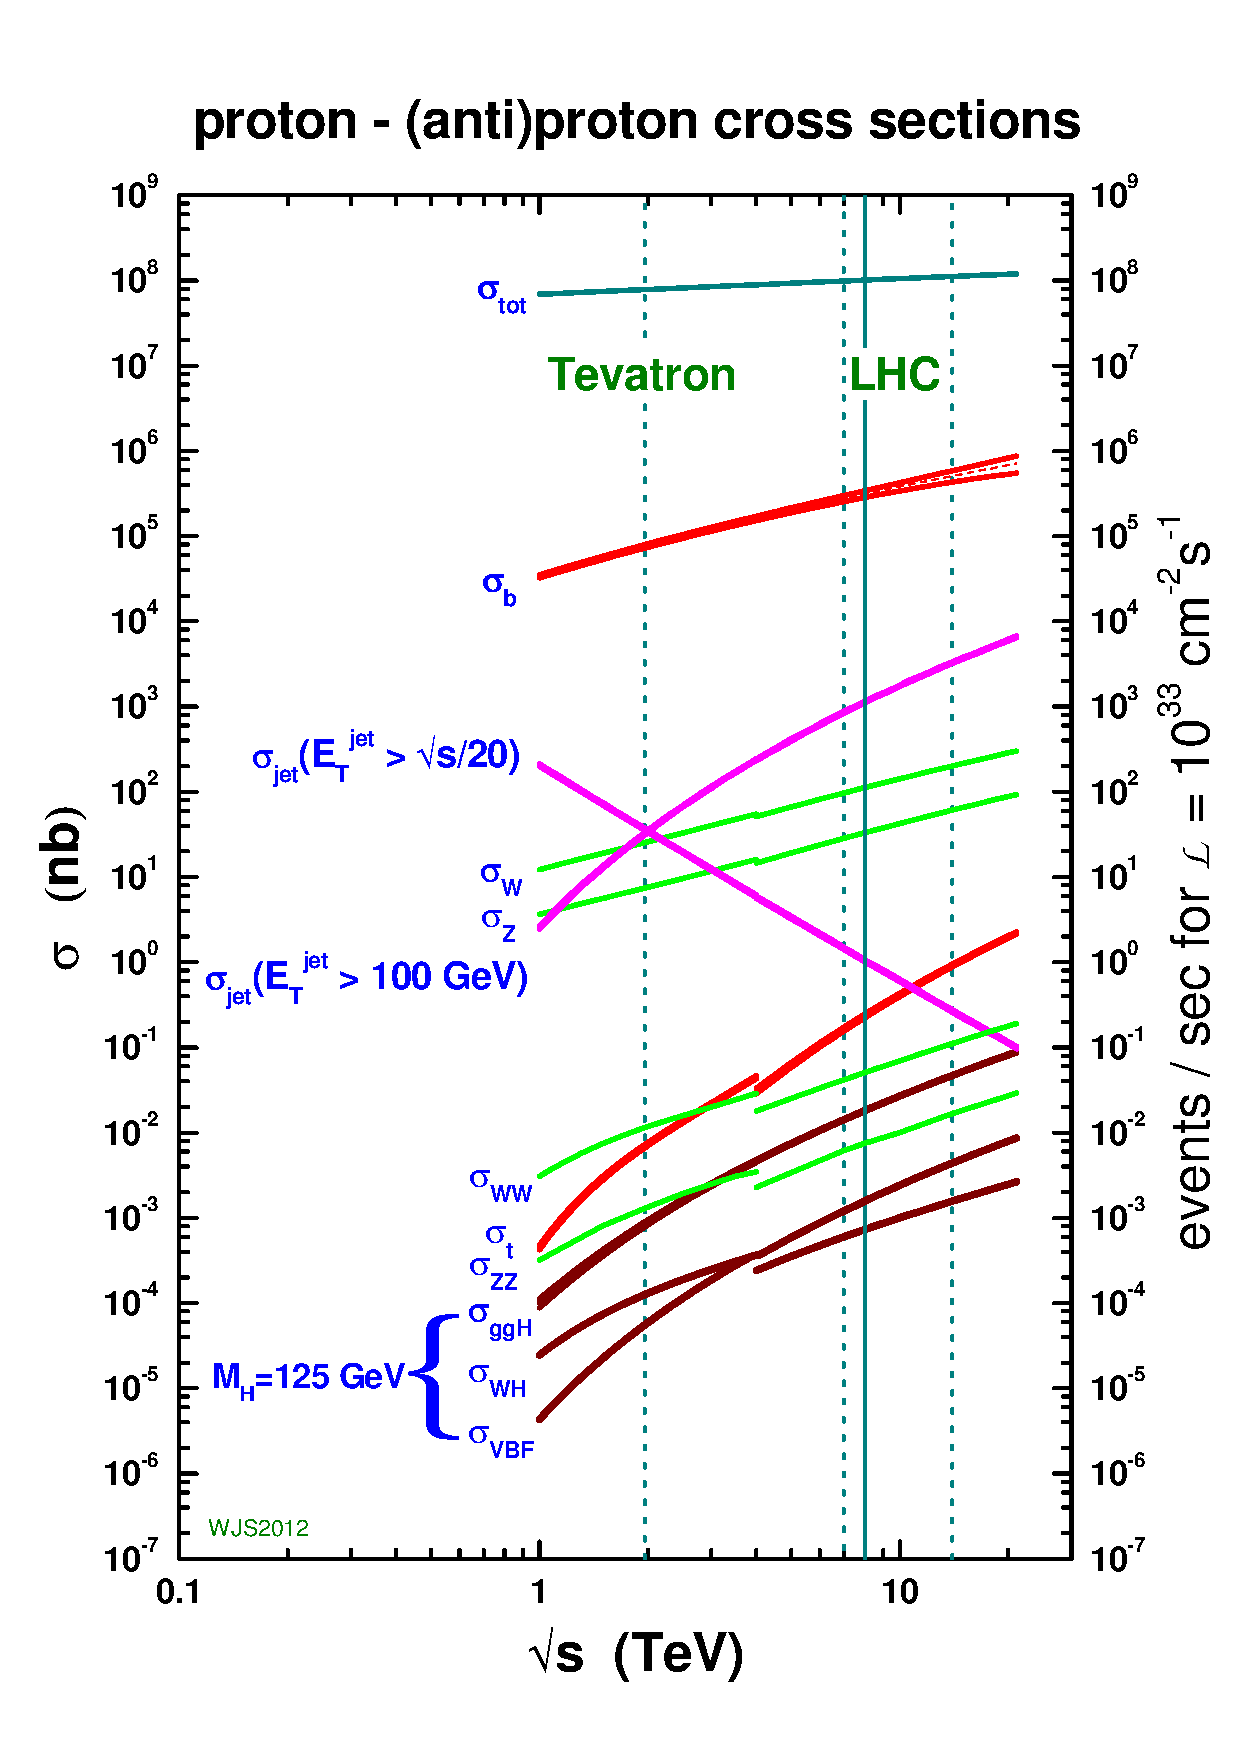
\includegraphics[width=.95\textwidth]{figures/protoncollisions/crosssections2012_v5.pdf}
    \caption{Cross-sections and event rates for various centre-of-mass energies \(\sqrt{s}\) in antiproton-proton (Tevatron, \(\sqrt{s} < \SI{4}{\giga\electronvolt}\)) and proton-proton (LHC, \(\sqrt{s} > \SI{4}{\giga\electronvolt}\)) collisions. The cross-sections have been calculated in perturbative QCD at \NLO and \NNLO using the MSTW2008 PDF set~\cite{Martin2009}. Figure reproduced from Ref.~\cite{Stirling2012}.}
    \label{fig:pp:crosssections:overview}
\end{figure}


\section{Event simulation}
\label{sec:pp:evgen}
The processes of interest in \HepProcess{\Pp\Pp} collisions are simulated by Monte Carlo (MC) event generators~\cite{Buckley2011,Sjostrand2016}.
The matrix elements of the hard scattering process are computed in perturbative QCD at fixed orders in \(\alpha_{s}\) in a highly automated way, together with the corresponding phase-space parametrisations. Event generators describing hard processes are \MGMCatNLO~\cite{Alwall:2014hca} (providing \LO and \NLO accuracy in QCD) and \POWHEG~\cite{Alioli:2010xd} (providing \NLO accuracy in QCD). The PDFs are parametrised in the LHAPDF format~\cite{Buckley2015}.
The secondary emissions are described by parton showers. Potential overlap of the multiple softer emissions of the parton showers and the higher-order matrix elements is resolved by matching and merging prescriptions.

The three general-purpose event generators \SHERPA~\cite{Gleisberg:2008ta}, \HERWIG~\cite{Bellm:2015jjp}, and \PYTHIA~\cite{Sjostrand:2014zea} provide combined descriptions of hard processes interfaced with parton showers. In particular, the \HERWIG and \PYTHIA generators can be interfaced with \MGMCatNLO or \POWHEG to supplement the parton shower description.

Finally, the interactions of final state particles with the ATLAS detector are simulated with the GEANT4~\cite{Agostinelli:2002hh} simulation tool-kit to provide the detector response~\cite{SOFT-2010-01}. The resulting set of simulated collision events is processed in the same manner as observed data with the reconstruction and event selection software.


\section{Hadronic jets}
\label{sec:pp:jets}
The parton shower evolution is dominated by the emission of partons which are either soft or collinear with the outgoing partons. Consequentially, the emerging hadrons are distributed in localised collimated sprays, which are called jets. The intriguing feature of jets is the correspondence between the total momentum of the hadrons contained in a jet and that of the corresponding partons described by perturbative calculations. This correspondence allows inferring the properties of the hard scattering process from the detector signature produced by QCD jets.

Jets are no fundamental objects but are instead defined by a jet algorithm. A jet algorithm provides a prescription on how to construct jets from input objects. Thereby, the algorithms need to fulfil two tasks. First, they need to identify all potential jet constituents. Second, they need to define the jet's four-vector based on the information provided by the constituents. A jet algorithm is agnostic to the precise nature of the input objects as long they can be parametrised as four-vectors. Therefore, the input objects can be partons, hadrons or energy deposits in the detectors.

A jet algorithm must be well-defined in arbitrarily high orders of perturbation theory, which involve additional parton emissions, to allow the direct comparison of perturbative calculations with observations. A well-defined jet algorithm, therefore, needs to satisfy the requirements of collinear and infra-red safety: neither collinear splitting nor soft emissions should alter the result of the jet algorithm.

There are two categories of jet algorithms, which differ in their method of identifying the jet constituents.
Cone-based algorithms, such as thee SISCone algorithm~\cite{Salam2007}, are based on purely geometric considerations by defining a jet axis and associating all objects within a specific radius parameter. Sequential algorithms cluster and combine pairs of objects until all objects have been used.

The \(k_{\text{T}}\) algorithms are a family of sequential algorithms, which satisfy the requirements of collinear and infra-red safety and are successfully employed at the Large Hadron Collider experiments.
They iteratively group objects \(i\) and \(j\) (referred to as pseudo-jets) into jets, using the two generalised distance measures in momentum space between two pseudo-jets (\(d_{ij}\)) and a pseudo-jet and the beam (\(d_{iB}\))
\begin{align}
	d_{iB} &= (\pt)^{2p} \\
    d_{ij} &= \min{\left\{(p_{\text{T}, i})^{2p}, (p_{\text{T}, j})^{2p} \right\}} \times \frac{R_{ij}}{R_{0}},
\end{align}
which are based on the transverse momenta of the pseudo-jets \(p_{\text{T}, i}\) and on the distance between the two objects in the \(\eta\)-\(\varphi\)-plane \(R_{ij} = \sqrt{\Delta\eta^2 + \Delta\varphi^2}\).

The algorithm evaluates all possible \(d_{ij}\) and \(d_{iB}\) and identifies the smallest distance. If the smallest distance is between a pseudo-jet and the beam, the pseudo-jet is promoted to a jet and is added to the list of output objects. Otherwise, the two pseudo-jets are discarded, and a new pseudo-jet \(k\) whose kinematic properties are based on their vector sum is created. This step is repeated until all pseudo-jets have been promoted to jets.

The parameter \(p\) defines the type of jet algorithm in the \(k_{\text{T}}\) family:
\begin{itemize}
	\item \(k_{\text{T}}\) algorithm (\(p = 1\))~\cite{Catani1993,Ellis1993}
	\item Cambridge/Aachen algorithm (\(p = 0\))~\cite{Dokshitzer1997,}
	\item \Antikt algorithm (\(p = -1\))~\cite{Cacciari2008}
\end{itemize}

The jet area can be determined by populating the \(\eta\)-\(\varphi\)-plane of an event with ghost particles, which have infinitely small momentum~\cite{Cacciari2008-2}. As the \(k_{\text{T}}\) algorithms are collinear and infra-red safe, the reconstructed jets are not changed by the addition of ghost particles. However, the association of the ghost particles with jets allows inferring the jet catchment area.

\Cref{fig:pp:jets:algorithms} shows a comparison of the resulting jet areas for the three algorithms of the \(k_{\text{T}}\) family and the SISCone algorithm. The \(k_{\text{T}}\) and Cambridge/Aachen algorithms produce jets with more irregular jet shapes, while the SISCone and \antikt algorithms have more regular jet shapes.

The \antikt algorithm, which is used as the standard jet algorithm in this dissertation, is collinear and infra-red safe and provides jets with a nearly conical shape at excellent reconstruction efficiency. Depending on the use-case, a different radius parameter is used for the jet reconstruction. The jet algorithms are implemented in the FastJet package~\cite{Cacciari2012}.

\begin{figure}[htbp]
    \centering
    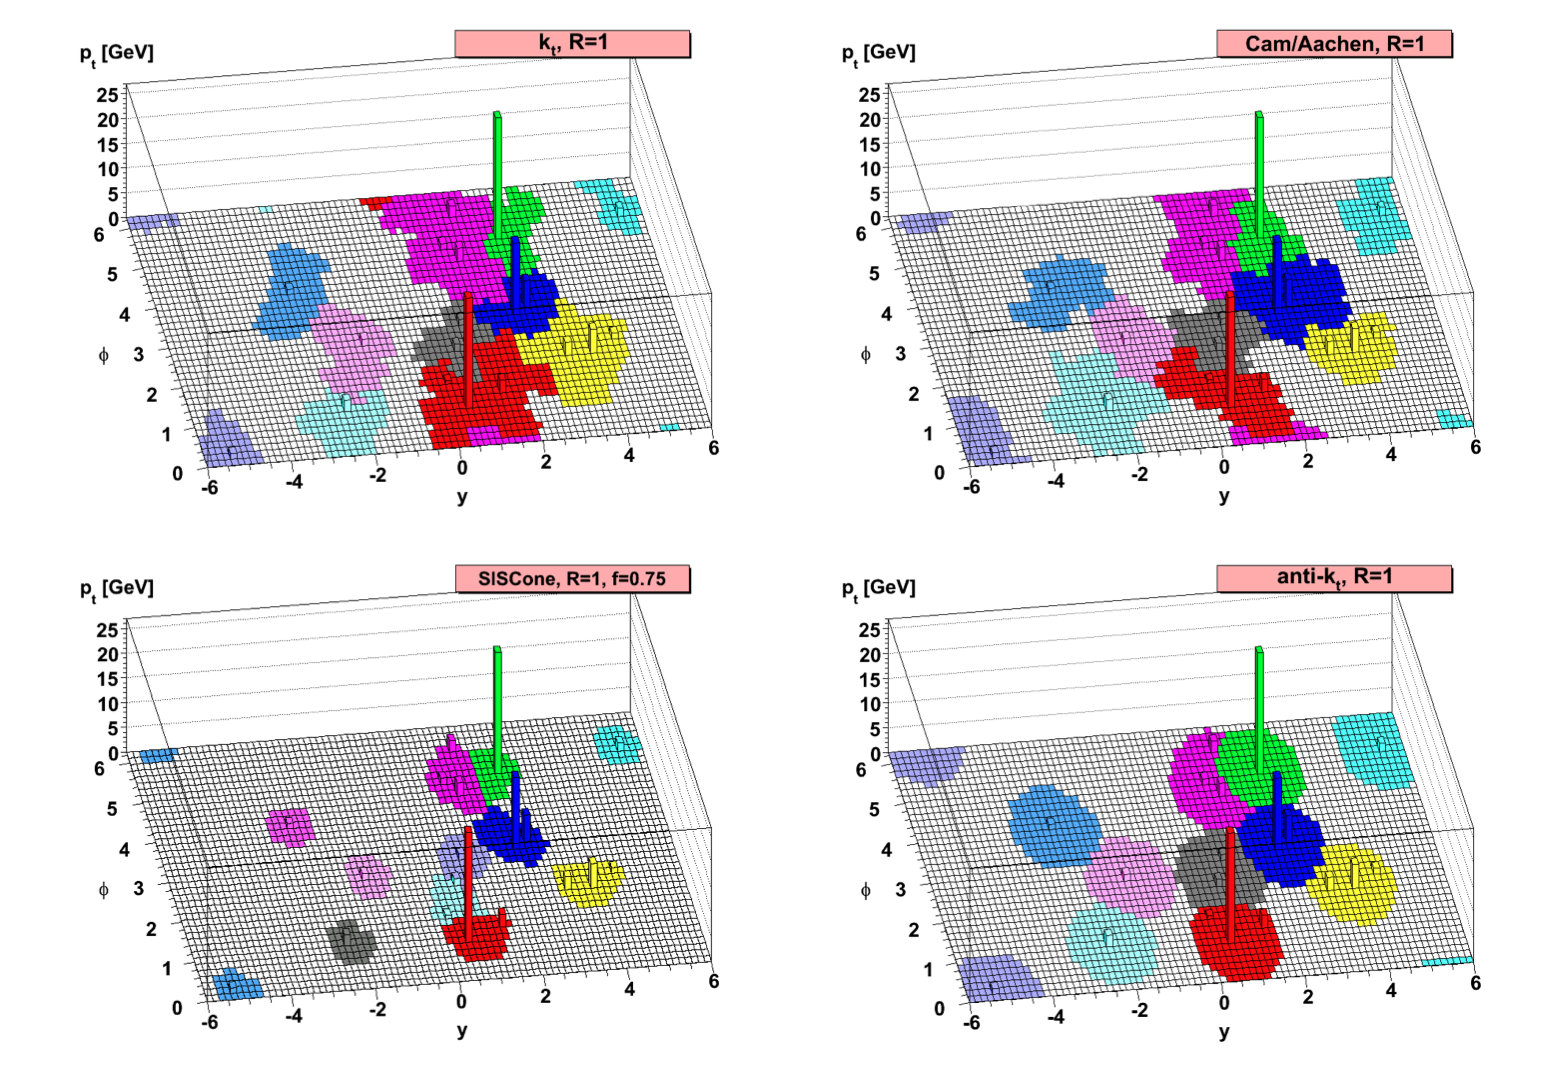
\includegraphics[width=.95\textwidth]{figures/protoncollisions/jetalgorithms.png}
    \caption{Clustering of a sample parton-level event with four different jet algorithms, illustrated by the active catchment area of the resulting hard jets. Figure reproduced from Ref.~\cite{Cacciari2008}.}
    \label{fig:pp:jets:algorithms}
\end{figure}
